\section{Directory service}

	A Directory service is a software system that stores, organises and provides access to a hierarchical database known as a Directory Information Base (DIB).  
	This Directory Information Base (DIB) is stored as object classes with each named attribute mapped to 
	one or more values. 
	\newline
	\newline
	These object classes consisting of Organisational Units (OU), Common Names (CN) etc. are identified by a Distinguished Name (DN).  
	A distinguished name is a concatenation of these attributes from a series of entries.  A Relative Distinguished Name (RDN) is the 
	tree along the path from the root to the named entry.  In the below example we have introduced more of the grammar associated with 
	a Directory Information Base (DIB) look up as well as the syntax.  
	\newline
	\newline
	The Distinguished Name (DN) at the beginning followed by the look up in right to left order.   As that of a Fully Qualified Domain 
	Name (FQDN) www.csis.ul.ie, the top of the tree is IE followed by UL, CSIS and so on.  In Fig. \ref{fig:DirectoryInformationBaseLookup} 
	for illustrative purposes I have ordered it from left to right, as this is how most people visualise it. 
	\newline

	\begin{center}
	�DN:  cn=J.J Collins + uid=j.jcollins, ou=Lecturers, dc=ul, dc=ie�
	\end{center}
	  
	\vspace{5mm}
	\begin{figure}[h!]
		\centering
		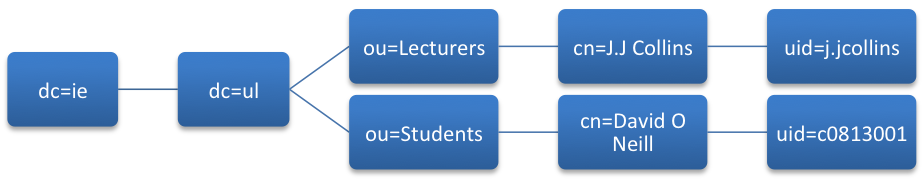
\includegraphics{pages/chapter1/figures/diblookup.png}
		\caption{Directory Information Base Lookup}
		\label{fig:DirectoryInformationBaseLookup}
	\end{figure} 		

	In this diagram we can identify five separate Relative Distinguished Names (RDN). 
	\newline 
	\newline
	RDN : dc=ie
	\newline
	RDN : dc=ul,dc=ie
	\newline
	RDN : ou=Lecturers, dc=ul,dc=ie
	\newline
	RDN : cn=J.JCollins,ou=Lecturers, dc=ul,dc=ie.
	\newline
	\newline  
	We can also identify an attribute signified by the plus symbol in the first example.
	\newline
	+ uid which is also an RDN.
	\newline
	\newline
	RDN : cn=J.JCollins + uid=j.jcollins,ou=Lecturers, dc=ul,dc=ie
	
\section{Domain Name System}
	
	The Domain Name System (DNS) is a hierarchical naming system for computers, services and any other resource identified by an 
	Internet Protocol (IP) address.  It associates names to nodes on a network known as uniform resource locators (URL).
	\newline
	\newline
	Before the advent of the Domain Name System (DNS), nodes relied on stored name/IP address pairs in a file called hosts.  
	When name lookups were requested, this text file was queried which resolved a name to an IP address.  As the networks grow in 
	size so did this hosts file and this became unsustainable.
	\newline
	\newline
	Two name spaces make up the domain hierarchy, the name address space and the Internet Protocol (IP) address.  The domain name server 
	maintains the mappings between the names and the Internet Protocol (IP) addresses.  Henceforth the domain name server stores records 
	such as address (A) records, name server (NS) records and mail exchanger (MX) records, as well some 30 other types.  When request from 
	a client is not found on a name server it requests it from its name servers thereby creating the physical hierarchy.
	\newline
	\newline
	Clients make requests to the name server using its Internet Protocol (IP) address.  These requests are sent to the server on 
	port 53 in a similar fashion to the way a host would query the hosts file.  The server receives the name request, performs the 
	look up and sends the Internet Protocol (IP) address pair mapping back to the client. 
	\newline
	\newline
	This process is further facilitated by the Dynamic Host Configuration Protocol (DHCP) which provides dynamic Internet Protocol (IP)
	assignments to requesting clients.  A Dynamic Host Configuration Protocol (DHCP) client running on a client machine broadcast a 
	request to 255.255.255.255 that is reserved for broadcast traffic. 
	\newline
	\newline 
	The Dynamic Host Configuration Protocol (DHCP) server listening for this broadcast traffic sends a response using the same method back 
	to the client consisting of an Internet Protocol (IP) address, a gateway address which is the host that joins to two networks together, 
	the broadcast address for the network and the domain name servers that the client can query for name resolving.
	\newline
	\newline
	The domain name space is split up logically in zones beginning at the root zone.  The sub zones are name spaces which Internet 
	Corporation for Assigned Names and Numbers (ICANN) has delegated administrative responsibility.
	\newline
	\newline
	Domain names are split up labels concatenated by full stops.  For example the right most label in the Fully Qualified Domain 
	Name (FQDN) \url{www.csis.ul.ie} being IE represents the top-level of the hierarchy to which authority has been delegated to Ireland's Domain 
	Registry (IEDR).
	\newline
	
	\begin{figurehere}
		\centering
		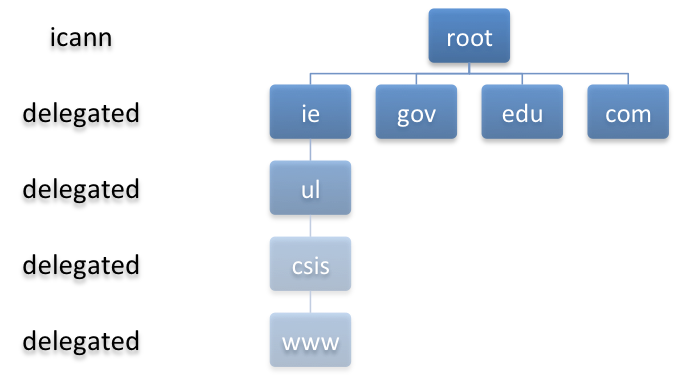
\includegraphics[scale=0.8]{pages/chapter1/figures/dnshier.png}
		\caption{Domain name system hierarchy}
	\end{figurehere}
	
	\vspace{5mm}
	
\section{X.500 Specification}	
	
	The X.500 specification is an amalgamation of computer networking standards for electronic directory services.  These standards 
	built upon Open Systems Interconnect (OSI) networking stack were the first approved implementation of the directory services.  
	The X.500 originally consisted of four main protocols, Directory Access Protocol (DAP), the Directory System Protocol (DSP), 
	the Directory Information Shadowing Protocol (DISP) and the Directory Operational Bindings Management Protocol (DOP).
	\newline
	\newline
	The Directory Access Protocol (DAP) or X.511 standard promulgated in 1998 by Open Systems Interconnect (OSI) is used by client 
	computers as a means of querying the directory services.  The query operations including bind, read, list, search, add, compare 
	modify and delete.  This protocol has long since been abandoned in favor of use of the Lightweight Directory Access Protocol (LDAP) 
	which was implemented using the transmission control protocol/internet protocol (TCP/IP), which supports extensibility as well as 
	introducing extensive error handling.  
	\newline
	\newline 
	The Lightweight Directory Access Protocol (LDAP) introduced amongst the most relevant advancements, Transport Later Security (TLS), 
	the abandon operation allowing the client server to abandon a request and the Extended Operation used to define other operations.
	Standalone servers soon followed supporting both the Lightweight Directory Access Protocol (LDAP) and Directory Access Protocol (DAP).  
	The next most prominent component of the X.500 specification was the Directory Services Protocol (DSP), which outlines the 
	communication specification between the Directory Services Agent (DSA) and the Directory User Agent (DUA).   The directory services 
	protocol controls the interaction between the user agents (clients) and the Services agent (server).
	\newline
	\newline
	The Directory Information Shadowing Protocol (DISP) described in the X.525 and X.519 specifications outlines the protocols and 
	procedures for the replication of directory information.  Replication being the act of copying from one Directory Services Agent (DSA) 
	to another.  This operation is generally achieved with the man in the middle approach (chaining and referrals), this ensures 
	synchronisation of data and reduces mismatch between Directory Services Agent''s (DSA) shown below.
	\newline

	\begin{figurehere}
		\centering
		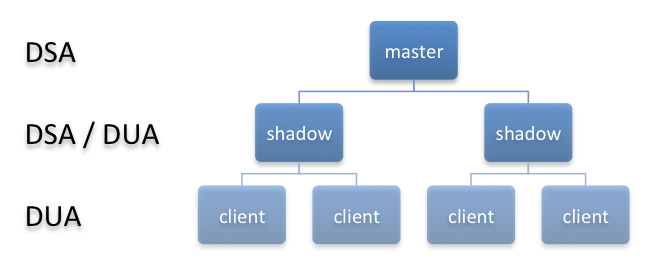
\includegraphics[scale=0.8]{pages/chapter1/figures/x500shadow.png}
		\caption{X.500 master and shadow servers}
	\end{figurehere}
		
	\vspace{5mm}
	
	
	The Directory Operational Bindings Management Protocol (DOP) was proposed to deal with the problem of multiple Directory Services 
	Agent''s (DSA); where no clear defined master could be identified.  Unlike the previous example of chaining and referrals the 
	relationship is clear.  
	\newline
	\newline 
	A shadow holds a subset of the master directory.  If the shadow does not have some information is refers it to the master.  
	But what if we have more than one master?  There is no clear chain of responsibility.   Therefore a relationship of responsibility 
	between the co-operating Directory Services Agent''s (DSA) must be established.  
	\newline
	\newline
	Two different types of operational binding were standardised, the Hierarchical Operational Binding (HOB) and the Shadow Operational 
	Binding (SOB).  These binding states allowed for the disjoint parts of a directory services to conglomerate seamlessly, aware of 
	what each other''s responsibilities were.  Consider the below figure.
	\newline
	
	\begin{figurehere}
		\centering
		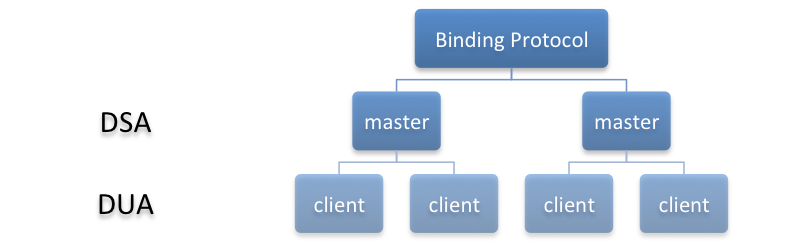
\includegraphics[scale=0.8]{pages/chapter1/figures/x500binding.png}
		\caption{X.500 binding protocol}
	\end{figurehere}
	
\section{Network Information Services}
		
	Network Information Services (NIS) previously known as Yellow Pages, is a client server directory services technology used for 
	network logins.   The Network Information Services (NIS) server (ypserv) distributes maps of resources, typically 
	Network File System (NFS) shares on a network as well as the contents of ``/etc/passwd'', ``/etc/shadow'' and ``/etc/group''.  
	\newline
	\newline
	A client bound to the server using the (ypbind) client automatically binds at boot.  When I user attempts a login on a client a 
	machine the Pluggable Authentication Module (PAM) loads the authentication modules in the order defined in the file 
	``/etc/nsswtich.conf'',  For eg. ``passwd: files NIS LDAP''.
	\newline
	\newline
	If the login information is not found in the local ``/etc/passwd'' file, the Pluggable Authentication Module (PAM) loads the next 
	login module in this case defined as ``NIS''.
	\newline
	\newline
	The maps distributed by (ypserv) are then checked and if the user is found authenticated, if not it then fails onto the next 
	authentication module until eventually failing to login and subsequently notifying the user.
	\newline
	\newline
	As previously mentioned one of the maps provided by Network Information Services (NIS) being Network File System (NFS) shares are 
	typically also used during the login process.  One of the secondary objectives of Network Information Services (NIS) is to make 
	available user resources on any networked machine they login to.  
	\newline
	\newline
	This is done using these maps and another application called ``autofs'' or ``automount''.  This map of shares defines the location 
	of a user''s home directory in the form of the local mount point and the network resource location where is home files are kept. 
	For example ``/home/dave   10.1.1.1:/home/dave''.
	\newline
	\newline
	Active Directory is a directory service technology created by Microsoft and is included with Windows Server.  Active Directory 
	serves primarily as a network administration and security backbone, but also provides advanced configuration of client machines 
	in the form of group policy, which is highly sought after in the Linux community and the motivation of this project.
	\newline
	\newline
	The structure of Active Directory is similar to that of the X.500 structure when multiple master domains are present.  
	These levels are logically divided into Forests, Tree and domains.  A tree being the most common implementation of organisations 
	Directory Services architecture is a collection of domains in contiguous space with an implicit transitive trust hierarchy. 
	\newline
	\newline 
	For example, Intel Corporation''s tree is split into five domains.  Each domain represents a region in the world.  If I user from 
	the greater Europe region attempts to access a machine in the American region, the target machine asks the domain controller for 
	that region for authorisation of the users account.  As the account does not exist in the American domain the domain controller 
	transitions the login request to the European domain controller which authorises the login, envisioning the trust.  The authorisation 
	is then cached on the American domain controller for later login requests.
	\newline
	\newline
	The domains themselves are further sub divided into Organisational Units.  Typically computer objects are grouped together and 
	user accounts are grouped together.  These organisational units can be further sub divided into smaller units creating a 
	hierarchical structure.  Group policies as previously discussed in 1.1 are attached to these organisational units.  
	\newline
	\newline
	As default each organisational unit has a default policy associated with it.  This default policy attributes are not configured as 
	default, meaning nothing will be modified on the target machine or adjusted on a users account.  An administrator then modifies 
	this policy, which is applied to the hierarchy top down in an inherited fashion.  A top-level policy can be over ridden by a 
	sub-level policy allowing for granular control of the sub units without having to have repeated policies within the hierarchy.
	\newline
	\newline

	
	\vspace{-5mm}
	\begin{figure}[h!]
		\centering
		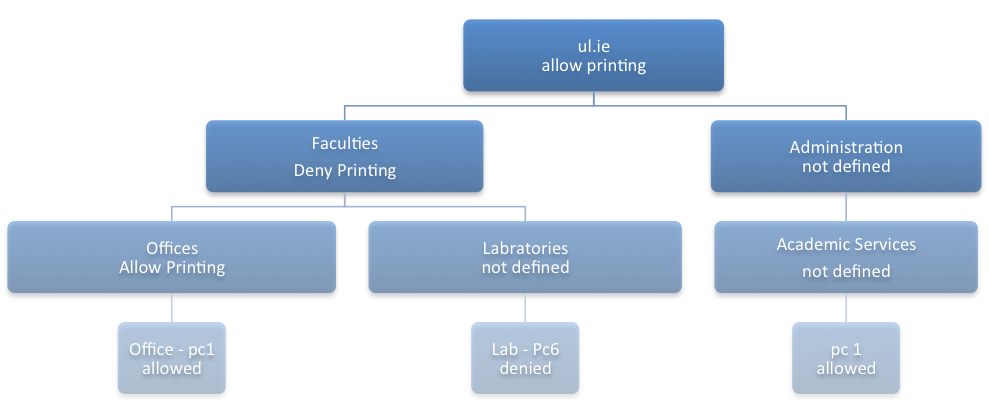
\includegraphics[scale=0.8]{pages/chapter1/figures/activedirectoryforest.png}
		\caption{Active directory domain hierarchy}
	\end{figure}
		
	\section{Linux Configuration Management}
	
	Many Linux configuration tools exist for both local and remote administration.  There has been varying degrees of success in 
	these solutions most notably with Cfengine.  
	\vspace{2mm}
	\subsection{Cfengine}
	One of the core issues with Cfengine is the requirement of the administrator to define policies via its Domain Specific Language (DSL) 
	similar to that of Javascript Object Notation (JSON).  This notation while catering for a wide variety of 
	configuration possibilities falls short of being truly easy to use as a result of the implementation''s huge vocabulary.  
	Furthermore it still requires expert knowledge in all the varying Linux systems, as each policy has to be coded by handed requiring 
	the administrator to aware of all the varying configurations and implementations of the client machines.  There is no front end or 
	point and click interface that comparable in any way of the of Windows Group Policy Editor.
	\vspace{2mm}
	\subsection{BCFG2}
	The second most notable configuration management application being BCFG2 provides software provisioning and configuration.  
	The policies are written in Extensible Mark-up Language (XML).  Each individual system and its configuration have to be addressed 
	once again requiring a domain expert.  The system is pluggable however unlike Cfengine allowing administrators to extend its 
	functionality.  No front end for the configuration of the policies exists other than industry standard tools for specifying 
	and validating Extensible Mark-up Language (XML). 
	\vspace{2mm}
	\subsection{Chef}
	Chef the third most notable Linux configuration manager distributes policies in the form of an internal Domain Specific Language (DSL) 
	(DSL).  Cookbooks, which define the policies, are short snippets of ruby code evaluated and executed by the client.  This solution 
	although very powerful and does not require the extensive learning of that of Cfengine but does however require the Administrator 
	to be familiar with the ruby general-purpose language.  The solution does not abstract the domain specific knowledge set and 
	still requires expert knowledge.

\newpage
	